\documentclass[twoside]{book}
\usepackage{graphicx}
\usepackage{amsmath}
\usepackage{amsthm}
\usepackage{amssymb}
\usepackage{xcolor}

% Bibliography
\usepackage{biblatex}
\addbibresource{bib.bib}
\DefineBibliographyStrings{english}{%
  bibliography = {References},
}

% Theorem Style
\theoremstyle{definition}
\newtheorem{example}{Example}[section]

\newcommand{\computation}{ \textcolor{violet}{\bigcirc\rightarrow} }

% \includeonly{computation/index}

\title{ The Elements of Intelligence
\thanks{This is the part one of a two-part project, as an update to the article \textit{Naturally} written in 2014, and the other part is \textit{A Guide to Life}}
\thanks{You can find more resources for this book at https://github.com/lin/eofi, and https://github.com/lin/guide for \textit{A Guide to Life}}
}
\author{Yingkui Lin}
\date{April 2019}

\begin{document}

  \frontmatter

  \maketitle

  \tableofcontents
  \chapter*{Preface}

To solve all problems, there is only one problem to solve, which is the problem of problem solving. So, why not solve it?

This book is a summary of my personal expedition to attack this problem. It tries to generalize and contain nearly everything I know about learning, solving and thinking. The simple assumption is that I believe we can simulate how human brain thinks and make it solve problems better than a gifted person. By saying all problems, what I really mean is that we can solve all problems  with certain level of complexity that's feasible to solve by a group of gifted human, like how to cure cancer and send human to Mars.

The programming language of this book is Javascript (ES6).

 The purpose of this book is to: 1. Layout the right structure. 2. Raise the right questions. 3. Rather solving it

 The analyse is two-folded, one for computation and mathematics, and another is human intelligence.

 We can't solve all the problems, the answer to some problems might hide in a tiny corner of the computational universe. But as we see, human brains are capable to lead us to many exiciting places, if we could mimic human brains brilliancy, that will be enough promising.

 To solve the problem, we start with an initial scan, and by assuming the answer is hidden within touch, a purposeless exploration starts. By increasing the searching area, we reach more and more, and explore deep and deep. In such solving techniques, at least in my own opinion we can mimic a human solver with intelligence score around 140 (top ~.25\% ). Maybe we still can't simulate how magicians like Newton and Gauss solve, but if we could have millions of MIT graduates as our solving slaves, how can we be more greedy at this time?

 to avoid philosophical and unnecessary blocks, we should agree on the purpose of this discuss, which is that we want to make engineering achievements. We want to make an intelligent computer who are smarter than us and willing to be our brain slave works day and night to satisfies our needs.

 That means any question that's unrelevant to this entrepreneur pursuit will be discarded.

 Why do we exist? Sorry, even I know the answer, it can't directly send me to the Mars. Does 2 exist? It works means lot to me than this unrelated question.

 So we care only one thing, does this help us to build a solver or not?

 Around 350 years ago, physics started and reached peak at early 20th century. Computer science started in 1936,

\noindent\makebox[\linewidth]{\rule{\textwidth}{1pt}}

The structure of this book:

1. The normal computation.

Beginning with distinguishability.

The last section will be loads of definitions.

2. The abstraction.

Beginning with tightness of distinguishability.

All sorts of pattern recognization feature extraction ability feature relationship all kinds of this related concepts

And end with a subsection of Layers of abstraction.

\[a \rightarrow \{ a\}  \rightarrow \{\{ a\}\}  \rightarrow \{\{\{ a\}\}\} \]

Then, The major part of this chapter should end with equivalence of computation.

This is a wonderful chapter. The computational Facts

\noindent\makebox[\linewidth]{\rule{\textwidth}{1pt}}

Now it's a late age of information and beginning age of intelligence, artificial intelligence will conquer the world where information can merely solve a small set of easier problems. In a foreseeable situation, all major disease will be cured. People can experience a simulation of any imaginable rules of the world, so real that you can't tell the difference from reality. You can sleep for 500 years, and resurrection at another planet. The possibility of life is unlimited.

The highlight of this whole book might be the emphasize on the importance of distinguishability.

The first chapter should be very short. Because it simply revisits the computation and computer system knowledges. Here we define distinguishability as a short introduction

The second should discuss distinguishability in details. And focusing on all kinds of abstract level computations.

The third chapter should discuss problems in details, how to define a problem and how to categorize problems in types. The hardest problem in this chapter in that

This book tries to generalize everything I know about learning and problem solving.

This is a book full of idiotic discuss, but through those simple to human yet complex to computer examples.

The grammar and vocabulary is a disaster, and I have to do this way so I don't waste too much computation power to less importance formating to the content.

Subjects lead to this result.

\begin{enumerate}
  \item Computer Systems
  \item Theory of Computation
  \item Computational Complexity Theory
  \item (Shannon) Information Theory
  \item Algorithmic Information Theory
  \item Pattern Recognization and Machine Learning
  \item Deep Learning
\end{enumerate}

If one person doesn't know about computer science, he doesn't understand the world very well, even true for giants like Eintein and Hilbert.

My understanding on computer science and mathematics.

This is a bold book. There are amazing books in various topics, both deep and brilliant. But I always want to read a book which have following features:

\begin{enumerate}
  \item accessable.
  \item talking about nearly everything.
  \item thinking in the highest level of abstraction.
\end{enumerate}

What I am not sure yet are:

\begin{enumerate}
  \item the importance of graph and linking
  \item the definition of problem
  \item why confident induction is working (solved!)
\end{enumerate}

\begin{enumerate}
  \item understanding how human thinks
  \item how to build a general artificial intelligence
  \item how things are related to real life situations
\end{enumerate}

Full of bad examples, cause searching the right examples requires too much time.

  % \addcontentsline{toc}{chapter}{\protect\numberline{}Preface}

  \mainmatter

  \chapter{Problems}

% introduction
\section{Problems}

To define a problem is defining a class at the same time.

To understand a problem is to know how to check whether one solution is correct or not.
\subsection{Verifying versus Searching}


% types of problems
\section{Types of Problems}
\subsection{Computational Problems}
\subsection{Learning Problems}
\subsection{Generic Problems}

% definition and properties of techniques
\section{Techniques}
The Classification of Techniques is a core concept in daily life.
\begin{figure}
  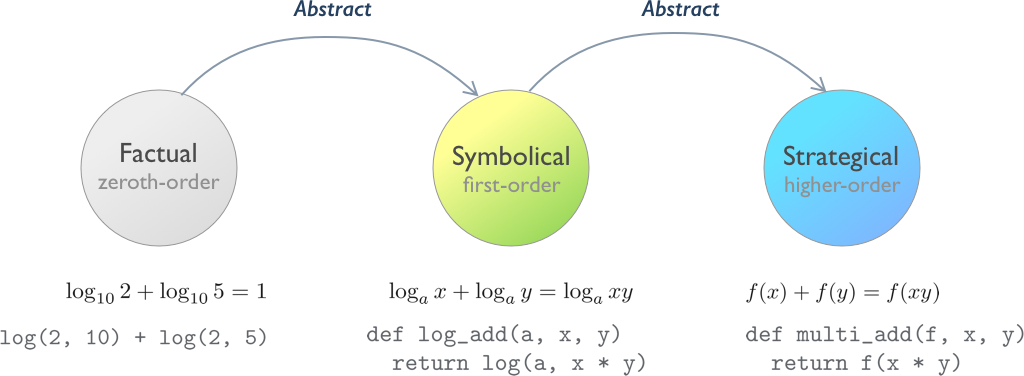
\includegraphics[width=\linewidth]{img/abstract-levels.png}
  \caption{Abstraction Levels}
  \label{fig:abstract-levels}
\end{figure}
\subsection{Robustness of Techniques}
\subsection{Frequency of Usage}
\subsection{Ad-Hoc versus Generic}
One phenominon that I experience a lot is the way people don't distinguish the difference between a ad-hoc technique and a generic technique. When a teacher or a guy present a way to solve a specific problem, few people will appreciate the robustness of this technique, that how well can you transfer your ability on this learning to another situations. But because of their inability to distinguish hardness and robustness, that leads to a dangerous place, that you have to learn too much techniques to cope with every problems, but you don't have enough time for learning these. And the teacher may think by doing an ad-hoc problem will lead to a better understanding for a more generic solving ability, which is vague. You don't learn too much on ad-hoc problems. You only know how to solve it in a nearby situations. The overall hint on a more generic solving strategies are often weak to recognize.

People don't know how to appreciate the robustness of techniques. Only can they find the dramatic changes of events. Even you simply press the button, you believe the underlining changes belongs to your smartness, well the main reason is the engineering behind the scene to smooth the user experience.
\subsection{Intensity of Signal}
\subsection{Trainability of Techniques}
Both the solving radius and the applicability.

% types of techniques
\section{Types of Techniques}
\subsection{Factual Techniques}
\subsection{Algorithmic Techniques}
\subsection{Strategic Techniques}
\subsection{Generic Techniques}
\subsection{Expansion Techniques}

  \chapter{Problems}

% introduction
\section{Problems}

To define a problem is defining a class at the same time.

To understand a problem is to know how to check whether one solution is correct or not.
\subsection{Verifying versus Searching}


% types of problems
\section{Types of Problems}
\subsection{Computational Problems}
\subsection{Learning Problems}
\subsection{Generic Problems}

% definition and properties of techniques
\section{Techniques}
The Classification of Techniques is a core concept in daily life.
\begin{figure}
  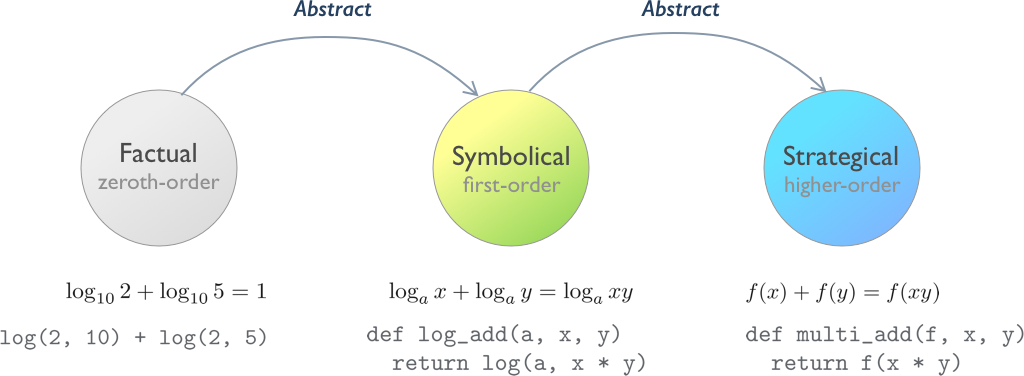
\includegraphics[width=\linewidth]{img/abstract-levels.png}
  \caption{Abstraction Levels}
  \label{fig:abstract-levels}
\end{figure}
\subsection{Robustness of Techniques}
\subsection{Frequency of Usage}
\subsection{Ad-Hoc versus Generic}
One phenominon that I experience a lot is the way people don't distinguish the difference between a ad-hoc technique and a generic technique. When a teacher or a guy present a way to solve a specific problem, few people will appreciate the robustness of this technique, that how well can you transfer your ability on this learning to another situations. But because of their inability to distinguish hardness and robustness, that leads to a dangerous place, that you have to learn too much techniques to cope with every problems, but you don't have enough time for learning these. And the teacher may think by doing an ad-hoc problem will lead to a better understanding for a more generic solving ability, which is vague. You don't learn too much on ad-hoc problems. You only know how to solve it in a nearby situations. The overall hint on a more generic solving strategies are often weak to recognize.

People don't know how to appreciate the robustness of techniques. Only can they find the dramatic changes of events. Even you simply press the button, you believe the underlining changes belongs to your smartness, well the main reason is the engineering behind the scene to smooth the user experience.
\subsection{Intensity of Signal}
\subsection{Trainability of Techniques}
Both the solving radius and the applicability.

% types of techniques
\section{Types of Techniques}
\subsection{Factual Techniques}
\subsection{Algorithmic Techniques}
\subsection{Strategic Techniques}
\subsection{Generic Techniques}
\subsection{Expansion Techniques}

  \chapter{Problems}

% introduction
\section{Problems}

To define a problem is defining a class at the same time.

To understand a problem is to know how to check whether one solution is correct or not.
\subsection{Verifying versus Searching}


% types of problems
\section{Types of Problems}
\subsection{Computational Problems}
\subsection{Learning Problems}
\subsection{Generic Problems}

% definition and properties of techniques
\section{Techniques}
The Classification of Techniques is a core concept in daily life.
\begin{figure}
  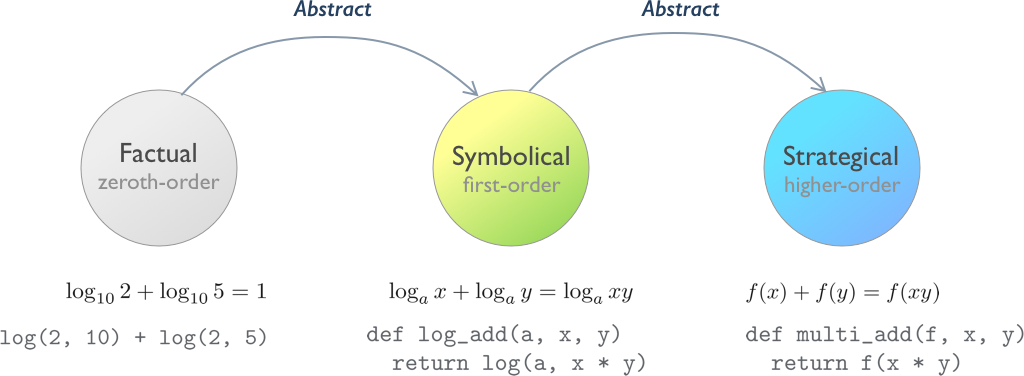
\includegraphics[width=\linewidth]{img/abstract-levels.png}
  \caption{Abstraction Levels}
  \label{fig:abstract-levels}
\end{figure}
\subsection{Robustness of Techniques}
\subsection{Frequency of Usage}
\subsection{Ad-Hoc versus Generic}
One phenominon that I experience a lot is the way people don't distinguish the difference between a ad-hoc technique and a generic technique. When a teacher or a guy present a way to solve a specific problem, few people will appreciate the robustness of this technique, that how well can you transfer your ability on this learning to another situations. But because of their inability to distinguish hardness and robustness, that leads to a dangerous place, that you have to learn too much techniques to cope with every problems, but you don't have enough time for learning these. And the teacher may think by doing an ad-hoc problem will lead to a better understanding for a more generic solving ability, which is vague. You don't learn too much on ad-hoc problems. You only know how to solve it in a nearby situations. The overall hint on a more generic solving strategies are often weak to recognize.

People don't know how to appreciate the robustness of techniques. Only can they find the dramatic changes of events. Even you simply press the button, you believe the underlining changes belongs to your smartness, well the main reason is the engineering behind the scene to smooth the user experience.
\subsection{Intensity of Signal}
\subsection{Trainability of Techniques}
Both the solving radius and the applicability.

% types of techniques
\section{Types of Techniques}
\subsection{Factual Techniques}
\subsection{Algorithmic Techniques}
\subsection{Strategic Techniques}
\subsection{Generic Techniques}
\subsection{Expansion Techniques}

  \chapter{Problems}

% introduction
\section{Problems}

To define a problem is defining a class at the same time.

To understand a problem is to know how to check whether one solution is correct or not.
\subsection{Verifying versus Searching}


% types of problems
\section{Types of Problems}
\subsection{Computational Problems}
\subsection{Learning Problems}
\subsection{Generic Problems}

% definition and properties of techniques
\section{Techniques}
The Classification of Techniques is a core concept in daily life.
\begin{figure}
  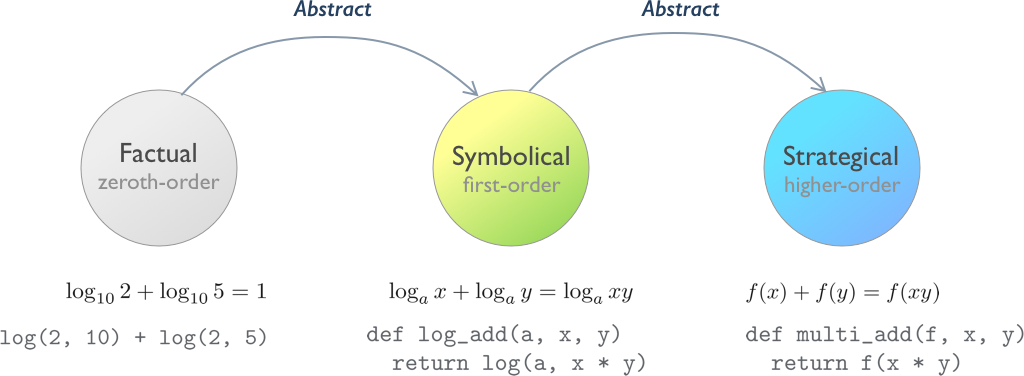
\includegraphics[width=\linewidth]{img/abstract-levels.png}
  \caption{Abstraction Levels}
  \label{fig:abstract-levels}
\end{figure}
\subsection{Robustness of Techniques}
\subsection{Frequency of Usage}
\subsection{Ad-Hoc versus Generic}
One phenominon that I experience a lot is the way people don't distinguish the difference between a ad-hoc technique and a generic technique. When a teacher or a guy present a way to solve a specific problem, few people will appreciate the robustness of this technique, that how well can you transfer your ability on this learning to another situations. But because of their inability to distinguish hardness and robustness, that leads to a dangerous place, that you have to learn too much techniques to cope with every problems, but you don't have enough time for learning these. And the teacher may think by doing an ad-hoc problem will lead to a better understanding for a more generic solving ability, which is vague. You don't learn too much on ad-hoc problems. You only know how to solve it in a nearby situations. The overall hint on a more generic solving strategies are often weak to recognize.

People don't know how to appreciate the robustness of techniques. Only can they find the dramatic changes of events. Even you simply press the button, you believe the underlining changes belongs to your smartness, well the main reason is the engineering behind the scene to smooth the user experience.
\subsection{Intensity of Signal}
\subsection{Trainability of Techniques}
Both the solving radius and the applicability.

% types of techniques
\section{Types of Techniques}
\subsection{Factual Techniques}
\subsection{Algorithmic Techniques}
\subsection{Strategic Techniques}
\subsection{Generic Techniques}
\subsection{Expansion Techniques}

  \chapter{Problems}

% introduction
\section{Problems}

To define a problem is defining a class at the same time.

To understand a problem is to know how to check whether one solution is correct or not.
\subsection{Verifying versus Searching}


% types of problems
\section{Types of Problems}
\subsection{Computational Problems}
\subsection{Learning Problems}
\subsection{Generic Problems}

% definition and properties of techniques
\section{Techniques}
The Classification of Techniques is a core concept in daily life.
\begin{figure}
  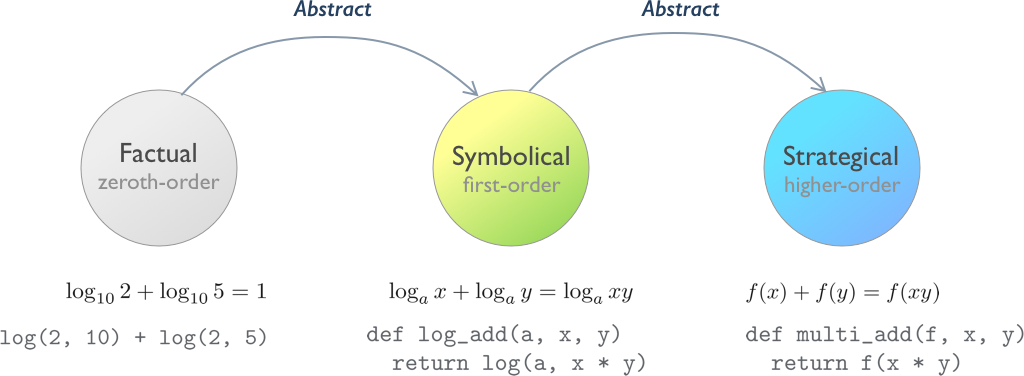
\includegraphics[width=\linewidth]{img/abstract-levels.png}
  \caption{Abstraction Levels}
  \label{fig:abstract-levels}
\end{figure}
\subsection{Robustness of Techniques}
\subsection{Frequency of Usage}
\subsection{Ad-Hoc versus Generic}
One phenominon that I experience a lot is the way people don't distinguish the difference between a ad-hoc technique and a generic technique. When a teacher or a guy present a way to solve a specific problem, few people will appreciate the robustness of this technique, that how well can you transfer your ability on this learning to another situations. But because of their inability to distinguish hardness and robustness, that leads to a dangerous place, that you have to learn too much techniques to cope with every problems, but you don't have enough time for learning these. And the teacher may think by doing an ad-hoc problem will lead to a better understanding for a more generic solving ability, which is vague. You don't learn too much on ad-hoc problems. You only know how to solve it in a nearby situations. The overall hint on a more generic solving strategies are often weak to recognize.

People don't know how to appreciate the robustness of techniques. Only can they find the dramatic changes of events. Even you simply press the button, you believe the underlining changes belongs to your smartness, well the main reason is the engineering behind the scene to smooth the user experience.
\subsection{Intensity of Signal}
\subsection{Trainability of Techniques}
Both the solving radius and the applicability.

% types of techniques
\section{Types of Techniques}
\subsection{Factual Techniques}
\subsection{Algorithmic Techniques}
\subsection{Strategic Techniques}
\subsection{Generic Techniques}
\subsection{Expansion Techniques}

  \chapter{Problems}

% introduction
\section{Problems}

To define a problem is defining a class at the same time.

To understand a problem is to know how to check whether one solution is correct or not.
\subsection{Verifying versus Searching}


% types of problems
\section{Types of Problems}
\subsection{Computational Problems}
\subsection{Learning Problems}
\subsection{Generic Problems}

% definition and properties of techniques
\section{Techniques}
The Classification of Techniques is a core concept in daily life.
\begin{figure}
  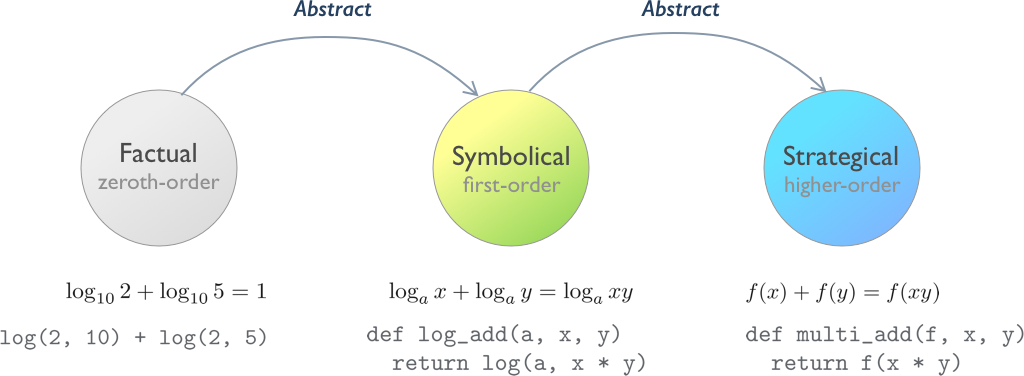
\includegraphics[width=\linewidth]{img/abstract-levels.png}
  \caption{Abstraction Levels}
  \label{fig:abstract-levels}
\end{figure}
\subsection{Robustness of Techniques}
\subsection{Frequency of Usage}
\subsection{Ad-Hoc versus Generic}
One phenominon that I experience a lot is the way people don't distinguish the difference between a ad-hoc technique and a generic technique. When a teacher or a guy present a way to solve a specific problem, few people will appreciate the robustness of this technique, that how well can you transfer your ability on this learning to another situations. But because of their inability to distinguish hardness and robustness, that leads to a dangerous place, that you have to learn too much techniques to cope with every problems, but you don't have enough time for learning these. And the teacher may think by doing an ad-hoc problem will lead to a better understanding for a more generic solving ability, which is vague. You don't learn too much on ad-hoc problems. You only know how to solve it in a nearby situations. The overall hint on a more generic solving strategies are often weak to recognize.

People don't know how to appreciate the robustness of techniques. Only can they find the dramatic changes of events. Even you simply press the button, you believe the underlining changes belongs to your smartness, well the main reason is the engineering behind the scene to smooth the user experience.
\subsection{Intensity of Signal}
\subsection{Trainability of Techniques}
Both the solving radius and the applicability.

% types of techniques
\section{Types of Techniques}
\subsection{Factual Techniques}
\subsection{Algorithmic Techniques}
\subsection{Strategic Techniques}
\subsection{Generic Techniques}
\subsection{Expansion Techniques}


  % \printbibliography[heading=bibintoc]

  \appendix

\end{document}
